% --------------------------------------------------------------
% This is all preamble stuff that you don't have to worry about.
% Head down to where it says "Start here"
% --------------------------------------------------------------

\documentclass[12pt]{article}

\usepackage[margin=1in]{geometry} 
\usepackage{amsmath,amsthm,amssymb}
\usepackage{color}
\usepackage{tikz, pgfplots}
\usepackage{graphicx}
\usepackage{epstopdf} %converting to PDF
\usepackage{subcaption}
\usepackage{listings}

\makeatletter

\renewcommand\section{\@startsection {section}{1}{\z@}%
	{-3.5ex \@plus -1ex \@minus -.2ex}%
	{2.3ex \@plus.2ex}%
	{\normalfont\large\bfseries}}% from \Large
\renewcommand\subsection{\@startsection{subsection}{2}{\z@}%
	{-3.25ex\@plus -1ex \@minus -.2ex}%
	{1.5ex \@plus .2ex}%
	{\normalfont\large\bfseries}}% from \large
\makeatother

\begin{document}
	
	% --------------------------------------------------------------
	%                         Start here
	% --------------------------------------------------------------
	
	%\renewcommand{\qedsymbol}{\filledbox}
	
	\title{\textbf{Advanced Topics in Machine Learning Exercise \#{5}}\\
	Universit{\"a}t Bern}%replace X with the appropriate number
	\author{{Lin Bai, 09935404}} %replace with your name
	
	\maketitle

	%%%%%%%%%%%%%%%%%%%%%%%%%%%%%%%%%%%%%%%%%%%%%%%%%%%%%%%%%%%%%%%%%%%%%%%%%%%%%%%%%%%
	%%%%%%   question 1
	%%%%%%%%%%%%%%%%%%%%%%%%%%%%%%%%%%%%%%%%%%%%%%%%%%%%%%%%%%%%%%%%%%%%%%%%%%%%%%%%%%%
	\section{Solution to question 1}
	\textbf{(a) What are the spatial dimensions of the outputs of all the layers from conv1 to pool5?}\\
	\\
	\noindent
	% https://github.com/dmlc/minerva/wiki/Walkthrough:-AlexNet
	Convolution layer output image size:\\
	$$Owidth = floor((width + 2*padW - kW) / dW + 1)$$
	$$Oheight = floor((width + 2*padH - kH) / dH+ 1)$$
	Max polling output image size:\\
	$$Owidth = round((width + 2*padW - kW) / dW + 1)$$
	$$Oheight = round((width + 2*padH - kH) / dH+ 1)$$
	\\
	\noindent
	The input image is 204x204x3.\\
	\textbf{conv1}: floor((204+2*0-11)/4+1)=49. So the output of \textbf{conv1} is 49x49x96.\\
	\textbf{pool1}: round((49+2*0-3)/2+1)=24. So the output \textbf{pool1} is 24x24x96.\\
	\textbf{conv2}: floor((24+2*2-5)/2+1)=12. So the output of \textbf{conv2} is 12x12x256.\\
	\textbf{pool2}: round((12+2*0-3)/2+1)=6. So the output \textbf{pool2} is 6x6x256.\\
	\textbf{conv3}: floor((6+2*1-3)/1+1)=6. So the output of \textbf{conv3} is 6x6x384.\\
	\textbf{conv4}: floor((6+2*1-3)/1+1)=6. So the output of \textbf{conv4} is 6x6x384.\\
	\textbf{conv5}: floor((6+2*1-3)/1+1)=6. So the output of \textbf{conv5} is 6x6x256.\\
	\textbf{pool5}: round((6+2*0-3)/1+1)=4. So the output \textbf{pool5} is 4x4x256.\\
	\\
	\noindent
	\textbf{(b) How many parameters does the network have? Show how you calculate the number of parameters of each layer separately. Which layer consists of most of the parameters?}\\
	\\
	\noindent
	\textbf{conv1}: (11*11)*3*96+96=34944\\
	\textbf{conv2}: (5*5)*96*256+256=614656\\
	\textbf{conv3}: (3*3)*256*384+384=885120\\
	\textbf{conv4}: (3*3)*384*384+384=1327488\\
	\textbf{conv5}: (3*3)*384*256+256=884992\\
	\textbf{conv4} has the most parameters.\\
	\\
	\noindent
	\textbf{(c) Calculate the receptive field of the neurons of the pool5 layer.}\\
	\\
	$$RF = ((fsize-1)*stride)+RF_{last}$$
	$$strides_i = strides_1 * strides_2 * ... * strides_{i-1}$$
	\textbf{conv1}: strides = 4,  RF = (11-1)*1+1=11\\
	\textbf{pool1}: strides = 8,  RF = (3-1)*4+11=19\\
	\textbf{conv2}: strides = 16, RF = (5-1)*8+19=51\\
	\textbf{pool2}: strides = 32, RF = (3-1)*16+51=83\\
	\textbf{conv3}: strides = 32, RF = (3-1)*32+83=147\\
	\textbf{conv4}: strides = 32, RF = (3-1)*32+147=211\\
	\textbf{conv5}: strides = 32, RF = (3-1)*32+211=275\\
	\textbf{pool5}: strides = 32, RF = (3-1)*32+275=339\\
	\\
	\noindent
	\textbf{(d) Suppose that you are given a pretrained AlexNet network. We feed the network with a new image and take the output of intermediate layers as features. Compute what input image sizes can be fed to the network, if we want to take the fc6 layer features. Is there such a limitation if we want to use convolutional layer activations as features?}\\
	\\
	
	
	%%%%%%%%%%%%%%%%%%%%%%%%%%%%%%%%%%%%%%%%%%%%%%%%%%%%%%%%%%%%%%%%%%%%%%%%%%%%%%%%%%%
	%%%%%%   question 2
	%%%%%%%%%%%%%%%%%%%%%%%%%%%%%%%%%%%%%%%%%%%%%%%%%%%%%%%%%%%%%%%%%%%%%%%%%%%%%%%%%%%
	\section{Solution to question 2}
	\textbf{(a) Given an input I with size 1xCxHxW and kernel K with size CxNxM , write the explicit formula for a convolution $Z_{ij}$ with stride s.}\\
	\\
	\textbf{(b) In Recurrent Neural Networks training, one potential issue is gradient vanishing, especially with long-term dependencies. Explain why this happens. Justify your answer mathematically.}\\
	\\
	From a simply neural network, each layer has only one neuron (shown below).\\
	\begin{figure}[htpb]
		\centering
		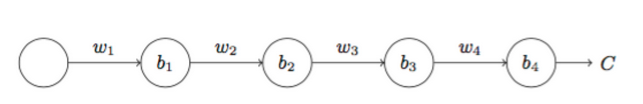
\includegraphics[width=0.9\textwidth]{images/1.png}
		\caption{}
	\end{figure}
	\\
	\noindent
	The gradient is 
	$$\frac{\partial C}{\partial b_1} = \sigma'(z_1)\omega_2\sigma'(z_2)\omega_3\sigma'(z_3)\omega_4\sigma'(z_4)\frac{\partial C}{\partial a_4}$$
	$$\frac{\partial C}{\partial b_1} = \sigma'(z_1)\times \omega_2 \sigma'(z_2) \times \omega_3 \times \sigma(z_3) \omega_4 \times \sigma(z_4) \times \frac{\partial C}{\partial a_4}$$
	\noindent
	If looking at the curve of sigmoid function
	\begin{figure}[htpb]
		\centering
		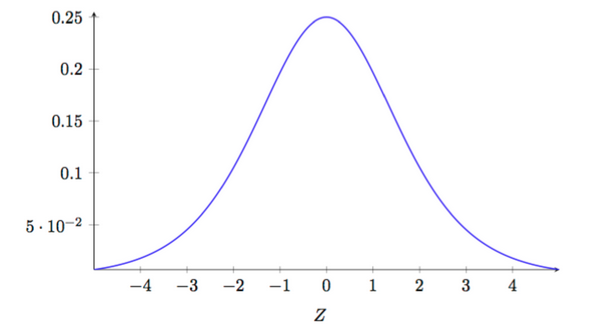
\includegraphics[width=0.7\textwidth]{images/2.png}
		\caption{}
	\end{figure}
	Its gradient reaches the highest when $\sigma'(0)=\frac{1}{4}$. Now, if we use standard method to the weights, then we will use the standard Gaussian distribution. Therefore, all the wights will fulfill $|\omega_j|<1$. Sum up what we have, we could find $\omega_j\sigma'_{(z_j)}<\frac{1}{4}$, and the result will decrease exponentially.\\
	\\
	We could compare the learning rate of the first layer and the third layer.\\
	$$\frac{\partial C}{\partial b_1} = \sigma'(z_1)\underbrace{\omega_2\sigma'(z_2)}_{<\frac{1}{4}}\underbrace{\omega_3\sigma'(z_3)}_{<\frac{1}{4}}\underbrace{\omega_4\sigma'(z_4)\frac{\partial C}{\partial a_4}}_{*}$$
	$$\frac{\partial C}{\partial b_3} = \omega_3\sigma'(z_3)\underbrace{\omega_4\sigma'(z_4)\frac{\partial C}{\partial a_4}}_{*}$$
	Where two $*$ in the formulas above are common terms.Comparing $\frac{\partial C}{\partial b_1}$ and $\frac{\partial C}{\partial b_3}$, we know $\frac{\partial C}{\partial b_1} \ll \frac{\partial C}{\partial b_3}$. Therefore, the reason of gradient vanishing is the constraint
	$$\omega_j\theta'(z_j)<\frac{1}{4}$$
	
	% --------------------------------------------------------------
	%     You don't have to mess with anything below this line.
	% --------------------------------------------------------------
	
\end{document}